\chapter{PPAR\texorpdfstring{$\gamma$}{gamma} M135 has the capacity to be insulin sensitizing
}\label{chap:chapter 2}

%%%%%%%%%%%%%%%%%%%%%%%%%%%%%%%%%%%%%%%%%%%%%%%%%%%%%%%%%%%%%%%%%%%%%%%%%%%%%%%%
\section{Introduction}
%%%%%%%%%%%%%%%%%%%%%%%%%%%%%%%%%%%%%%%%%%%%%%%%%%%%%%%%%%%%%%%%%%%%%%%%%%%%%%%%

The \(PPARG\) gene encodes PPAR$\gamma$, a nuclear hormone receptor that is a master regulator of adipocyte differentiation and is the molecular target of thiazolidinediones (TZDs), a class of drugs that decrease insulin resistance\cite{Tontonoz2008-pe,Yki-Jarvinen2004-ba}. TZDs are potent insulin sensitizers that treat type 2 diabetes, cardiovascular disease (CVD), and non-alcoholic fatty liver disease (NAFLD)\cite{Kernan2016-fd,Inzucchi2016-ni,Musso2017-xi}, but they cause serious side effects, including fluid retention\cite{Yki-Jarvinen2004-ba}. A novel isoform of PPAR$\gamma$, named PPAR$\gamma$ M135, was identified and characterized in Chapter 1. This isoform demonstrated increased transactivation potential in response to TZD treatment compared to wild-type PPAR$\gamma$2.

PPAR$\gamma$ M135 differs from canonical isoforms PPAR$\gamma$1 and PPAR$\gamma$2 with its lack of the autonomous activation-function domain 1 (AF-1); the DNA binding domain (DBD) and ligand binding domain (LBD) are present in all three isoforms. Multiple loss-of-function (LOF) mutations in \(PPARG\) occurring in the DBD and LBD have been shown to cause familial partial lipodystrophy type 3 (FPLD3), a Mendelian genetic syndrome characterized by insulin resistance, metabolic syndrome, and gluteofemoral fat loss\cite{Savage2003-wm,Agostini2006-hc,Broekema2019-nz}. These pathogenic FPLD3 mutations establish the clinical significance of the PPAR$\gamma$ DBD and LBD, but form the tip of the iceberg in human protein-coding variants found in \(PPARG\)\cite{Majithia2014-op}. In previous work, we have identified hundreds of protein-coding variants in \(PPARG\) occurring in all protein domains including the AF-1 domain\cite{Majithia2016-bm}. As with FPLD3, those that cause LOF in the DBD and LBD increased insulin resistance and type 2 diabetes risk. We observed no apparent clinical impact of LOF variants in the AF-1 domain, leaving in question its function in human metabolic health.

In this study, we expand on the insulin sensitizing activity of PPAR$\gamma$ M135. We find that PPAR$\gamma$ M135 demonstrates enhanced ligand-inducible transcriptional and functional activity compared to wild-type (WT) in a human preadipocyte cell line. To evaluate the clinical consequence of this model, we identified and analyzed human carriers of \(PPARG\) variants that impair AF-1 function, finding that these variants increase PPAR$\gamma$ function and decrease metabolic syndrome severity in people who carry them. Taken together, our study nominates AF-1 domain inhibition as a new targetable mechanism to activate PPAR$\gamma$.

%%%%%%%%%%%%%%%%%%%%%%%%%%%%%%%%%%%%%%%%%%%%%%%%%%%%%%%%%%%%%%%%%%%%%%%%%%%%%%%%
\section{Results}
%%%%%%%%%%%%%%%%%%%%%%%%%%%%%%%%%%%%%%%%%%%%%%%%%%%%%%%%%%%%%%%%%%%%%%%%%%%%%%%%

\subsection{Human preadipocytes that generate PPAR\texorpdfstring{$\gamma$}{gamma} M135 more potently upregulate target genes than WT preadipocytes}

As many of the major metabolic effects of \(PPARG\) on human physiology occur in adipocytes\cite{Majithia2014-op}, we evaluated if adipocytes could also generate PPAR$\gamma$ M135 and to what functional consequence. We targeted a human preadipocyte cell line (Simpson-Golabi-Behmel Syndrome (SGBS)\cite{Wabitsch2001-fx}) with disruptions in Exon 1, Exon 3, and a \(PPARG\) intron (Ex1-sgRNA2 cut site at hg38 chr3:12379716, Ex3-sgRNA chr3:12392733, and Int-sgRNA chr3:12363492, \textbf{Figure 2.1A}). The edited cells were treated with inducers of adipocyte differentiation and examined for PPAR$\gamma$ protein expression, target gene expression, and adipocyte differentiation efficiency. After four days of differentiation, we were able to detect both PPAR$\gamma$ WT and M135 in Exon 1 targeted cells, whereas Exon 3 targeted cells expressed no PPAR$\gamma$, and control cells only expressed WT PPAR$\gamma$ (\textbf{Figure 2.1B, C}). These results indicated that, like THP-1 macrophages, SGBS adipocytes are capable of alternatively generating PPAR$\gamma$ M135 in response to disruptive mutations targeted to Exon 1.

\clearpage
\begin{figure}[!ht]
    \centering
    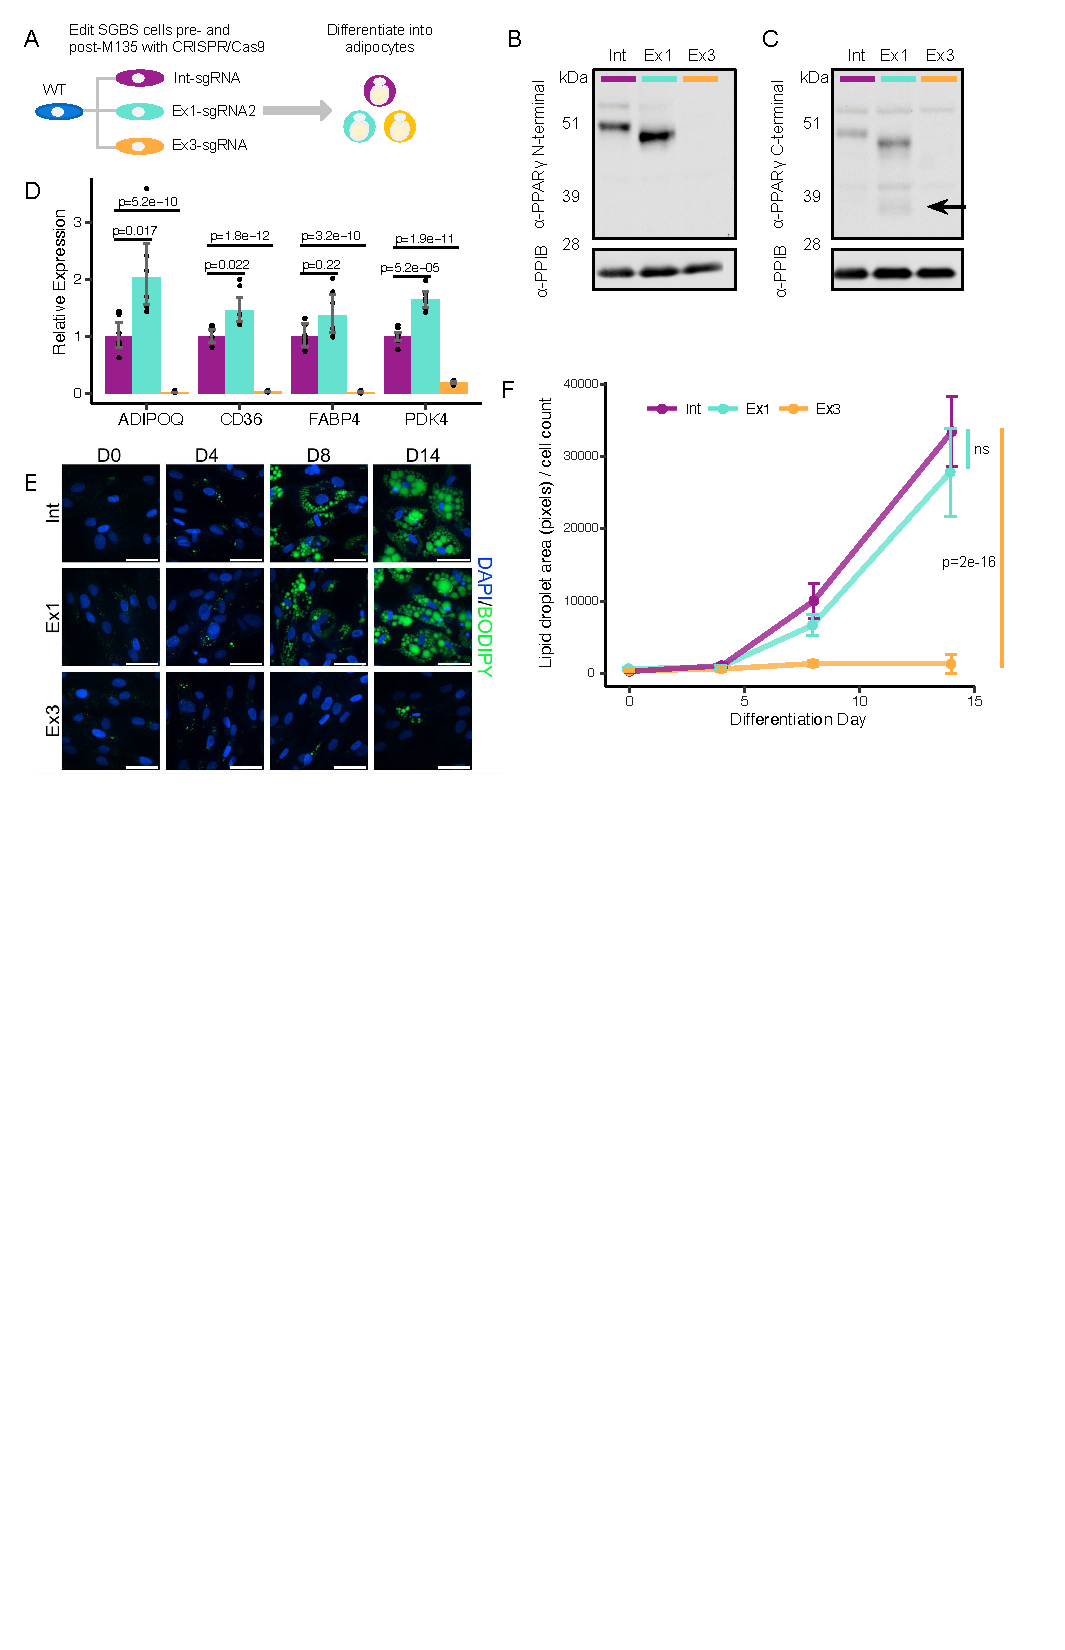
\includegraphics[width=\textwidth]{2_figures-and-files/Fig1.pdf}
    \caption[Human preadipocytes generate PPAR$\gamma$ M135 and more potently upregulate target genes than WT]{\textbf{Human preadipocytes generate PPAR$\gamma$ M135 and more potently upregulate target genes than WT.} \textbf{A.} Simpson-Golabi-Behmel Syndrome (SGBS) cells were transduced with a vector containing Cas9 and a sgRNA targeting \(PPARG\) Exon 1 (chr3:12379716), Exon 3 (chr3:12392733), or an intron (chr3:12363492). The preadipocytes were differentiated into adipocytes. \textbf{B,} \textbf{C.} Western blot for the N-terminus (B, left) and C-terminus (C, right) of PPAR$\gamma$ in SGBS preadipocytes treated with \(PPARG\) targeting constructs (A) at 4 days post-differentiation. The Ex1 targeted preadipocytes generate PPAR$\gamma$ M135 at 40 kDa (arrow), while the Ex3 targeted cells do not express any PPAR$\gamma$. Exon 1 targeted cells also express a band $\sim$50 kDA, consistent with translation initiation at PPAR$\gamma$ p.M53. \textbf{D.} Expression of PPAR$\gamma$ target genes at 4 days of differentiation by qPCR.\@ Ex1 targeted cells expressed higher levels of \(ADIPOQ\), \(CD36\), and \(PDK4\) compared to control. Ex3 edited cells minimally express all PPAR$\gamma$ target genes. N=6 replicates per sample, p-values from linear models of $\Delta$ Ct (see Methods for more details). \textbf{E,} \textbf{F.} Differentiation time-course for Int, Ex1, and Ex3 targeted SGBS cells at days 0, 4, 8, and 14. Cells were fixed and stored in PBS on their respective collection dates, stained on day 14 for nuclei (DAPI, blue) and lipids (BODIPY, green), and imaged. \textbf{E.} Imaged at 40x magnification. Ex1 SGBS differentiate on par with Int, and Ex3 SGBS do not accumulate lipids. Scale bar is 50 $\mu$m. \textbf{F.} Quantification of lipid accumulation in SGBS cells. The data was log-normalized and regressed against genotype and differentiation day to determine the effect of genotype. Ex1 was not different from Int (p=0.933), and Ex3 resulted in a significantly different pace (p = 2e-16).
    }\label{fig:PPARgamma M135 in human adipocytes}
\end{figure}
\clearpage

To evaluate the ability of preadipocytes expressing PPAR$\gamma$ M135 to activate PPAR$\gamma$ target genes, we queried gene expression of several targets during early adipocyte differentiation (\textbf{Figure 2.1D}). SGBS preadipocytes that express PPAR$\gamma$ M135 increase expression of \(CD36\) (p=0.022) and \(PDK4\) (p=5.2e-5) to a significantly greater extent than PPAR$\gamma$ WT expressing cells and showed a trend towards increased expression of \(FABP4\) (p=0.22). Furthermore, we examined adiponectin (\(ADIPOQ\)), an adipokine and PPAR$\gamma$ target specific to adipocytes\cite{Combs2002-sr}, and found it also to be significantly upregulated by PPAR$\gamma$ M135 expressing adipocytes (p=0.017) compared to WT (\textbf{Figure 2.1D}). Cells targeted at Exon 3, which expressed no PPAR$\gamma$, failed to upregulate the expression of any of these genes. 

Finally, we characterized the ability of PPAR$\gamma$ M135 expressing SGBS cells to mature into adipocytes and accumulate lipids during differentiation (\textbf{Figure 2.1E, F}). Exon 1 targeted, PPAR$\gamma$ M135 expressing SGBS differentiated and accumulated lipids at the same rate as control PPAR$\gamma$ WT expressing cells (p=0.933), whereas Exon 3 targeted cells had significantly reduced lipid accumulation (p=2e-16). These analyses show that like macrophages, human preadipocytes can generate the PPAR$\gamma$ M135 isoform, and the truncated isoform is fully functional in driving differentiation into mature, lipid-laden adipocytes.

\subsection{PPAR\texorpdfstring{$\gamma$}{gamma} M135 enhances adipocyte insulin response compared to WT}

To isolate the effect of PPAR$\gamma$ M135, we transduced P$\gamma$-/- SBGS cells (i.e. Ex3-sgRNA targeted cells) with doxycycline-inducible WT PPAR$\gamma$2 cDNA (SGBS P$\gamma$-/- +WT) or PPAR$\gamma$ M135 cDNA (SGBS P$\gamma$-/- +M135) transgenes and evaluated differentiation/ lipid accumulation and insulin response (\textbf{Figure 2.2A}). These cells only express PPAR$\gamma$ (WT or M135) when treated with doxycycline (\textbf{Figure 2.2B}) and differentiate to a similar degree only when PPAR$\gamma$ is induced (p=0.56, \textbf{Figure 2.2C, D}).

\clearpage
\begin{figure}[ht]
    \centering
    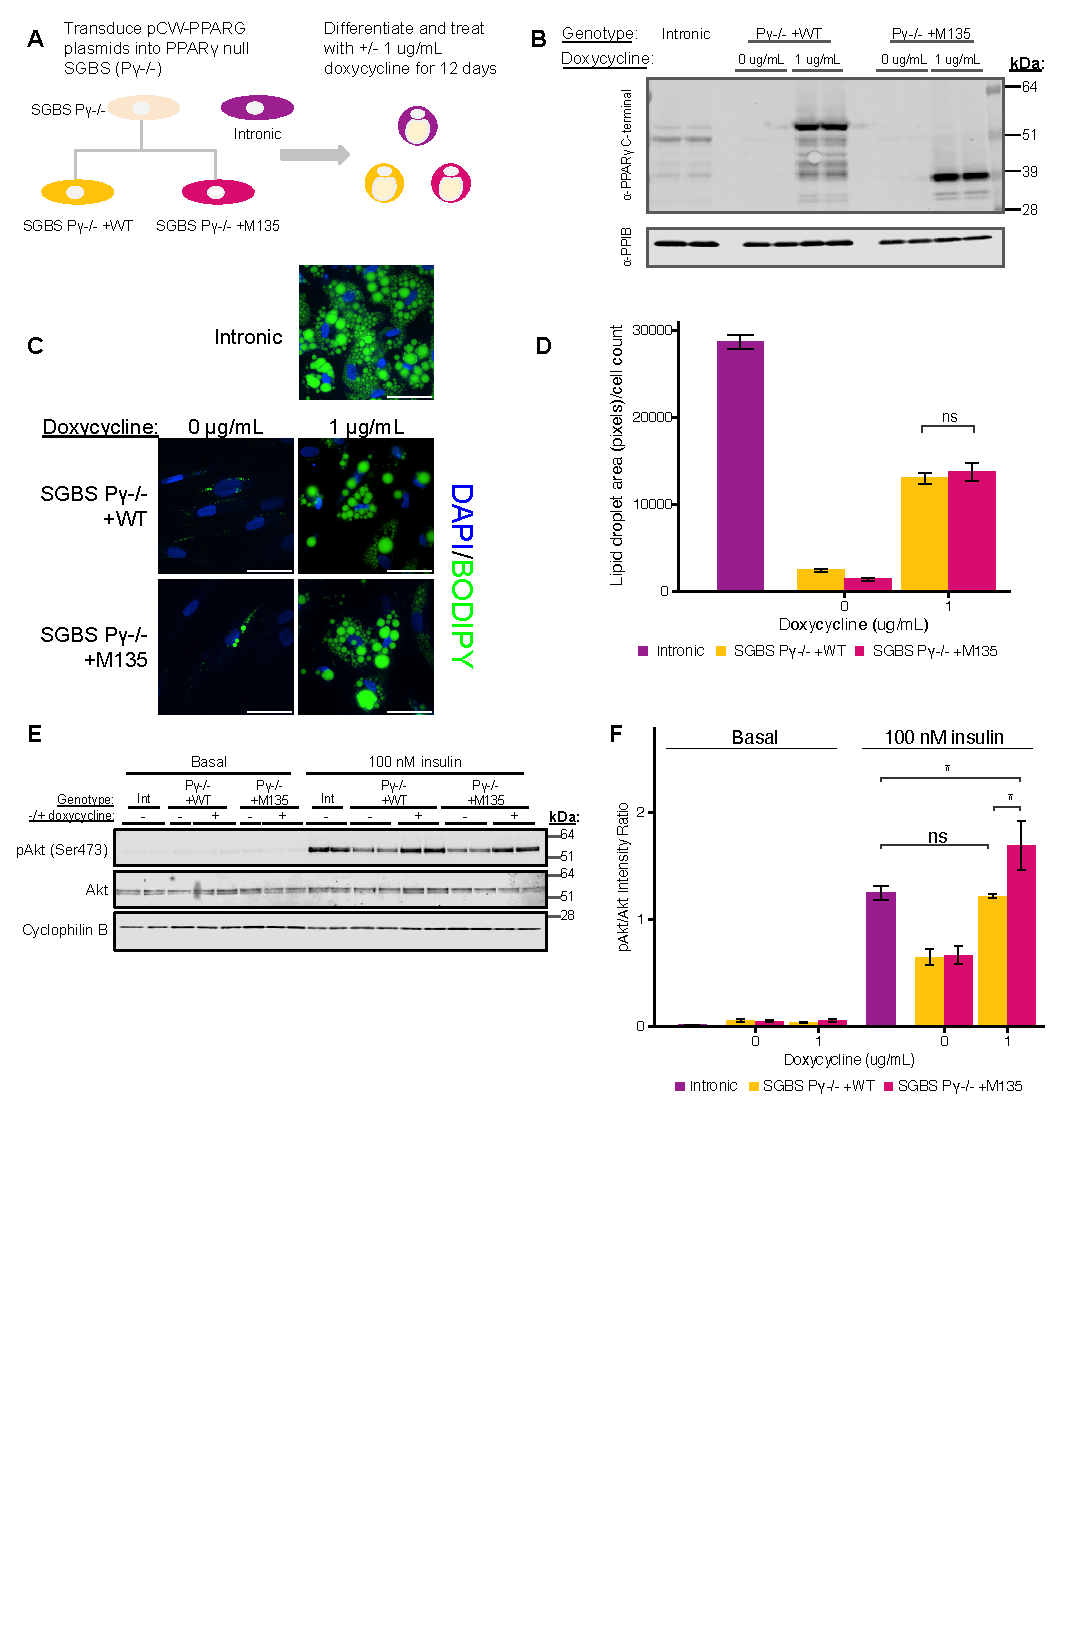
\includegraphics[width=0.8\textwidth]{2_figures-and-files/Fig2.pdf}
    \caption[PPAR$\gamma$ M135 enhances adipocyte insulin response compared to WT.]{\textbf{PPAR$\gamma$ M135 enhances adipocyte insulin response compared to WT.} \textbf{A.} SGBS P$\gamma$-/- cells were transduced with doxycycline-inducible vectors expressing PPARG WT and M135. The preadipocytes were differentiated and treated +/- doxycycline. \textbf{B.} PPAR$\gamma$ expression in the SGBS cells. SGBS P$\gamma$-/- cells with PPARG transgenes only express PPAR$\gamma$ when treated with doxycycline. \textbf{C,} \textbf{D.} Intronic, SGBS P$\gamma$-/- +WT, and SGBS P$\gamma$-/- +M135 cells were differentiated for 12 days, fixed, stained for nuclei (DAPI, blue) and lipid accumulation (BODIPY, green), and imaged. \textbf{C,} Imaged at 40x magnification. PPAR$\gamma$ M135 is sufficient to induce differentiation and lipid uptake in SGBS P$\gamma$-/- cells. Scale bar is 50 $\mu$m. \textbf{D.} Quantification of lipid accumulation. SGBS P$\gamma$-/- +M135 cells accumulate the same amount of lipids as SGBS P$\gamma$-/- +WT (n=12 images/well, 4 wells per genotype, p=0.56, t-test). \textbf{E,} \textbf{F.} Intronic, SGBS P$\gamma$-/- +WT, and SGBS P$\gamma$-/- +M135 cells were treated +/+ doxycycline, +/+ 100 nM insulin for 20 minutes and immunoblotted for phosphorylated Akt (pAkt) and total Akt (n=4 biological replicates). \textbf{E.} Representative immunoblot. \textbf{F.} The pAkt/Akt intensity ratios were significantly different across the conditions (ANOVA p=1.33e-13). Pairwise comparisons are highlighted between the 100 nM insulin stimulated samples for SGBS P$\gamma$-/- +M135 and SGBS P$\gamma$-/- +WT cells treated with 1 ug/mL doxycycline (Tukey HSD p=0.025, *), SGBS P$\gamma$-/- +M135 + doxycycline and Intronic (p=0.045, *), and SGBS P$\gamma$-/- +WT + doxycycline and Intronic (p=0.99, ns). 
    }\label{fig:PPARgamma M135 insulin response}
\end{figure}
\clearpage

To assess insulin response control (intronic), SGBS P$\gamma$-/- +WT and SGBS P$\gamma$-/- +M135 were differentiated, stimulated with insulin and immunoblotted for phosphorylated Akt (S473; pAkt) and total Akt. In response to insulin all cell lines phosphorylate Akt and the response is augmented in doxycycline treated SGBS P$\gamma$-/- +WT and SGBS P$\gamma$-/- +M135 (ANOVA p=1.33e-13, Tukey HSD $\mathrm{p}_{\mathrm{WT, doxycycline}}$=3.67e-8, $\mathrm{p}_{\mathrm{M135, doxycycline}}$=3.43e-11, \textbf{Figure 2.2E, F}). Notably, PPAR$\gamma$ M135 expressing adipocytes show increased insulin stimulated AKT phosphorylation compared to both WT(p=0.025) and control SGBS (p=0.045), indicating an enhanced insulin response.

\subsection{Missense mutations that impair AF-1 function increase PPAR\texorpdfstring{$\gamma$}{gamma} transactivation and may protect against metabolic syndrome in human carriers}

Next, we sought to evaluate the potential in vivo consequence of nonsense mutations in the \(PPARG\) sequence prior to chr3:12381414 by identifying human carriers of such mutations and performing genotype:phenotype correlation under the hypothesis that carriers would not exhibit insulin resistance given the enhanced molecular activity of PPAR$\gamma$ M135 from AF-1 domain deletion. Across biobanks and databases comprising over 1.2 million individuals with sequencing at the \(PPARG\) locus, we only found seven carriers of nonsense mutations prior to chr3:12381414 (\textbf{Table B.1}). Among these, two had no evidence of metabolic syndrome or insulin resistance past 50 years of age, one had type 2 diabetes, but no ascertainment of insulin resistance or metabolic syndrome, and four had no available phenotypic information.

As the number of human pre-M135 nonsense mutation carriers was insufficient to make robust inferences, we turned to carriers of \(PPARG\) missense variants to test the hypothesis that genetic variants abrogating AF-1 domain function would enhance PPAR$\gamma$ activity and thereby increase insulin sensitivity in vivo (\textbf{Figure 2.3A}). While missense variants are not equal to having the M135 isoform, they can model how disruptions to the AF-1 domain affect PPAR$\gamma$ activity in vivo. We rationalized this hypothesis based on recent data that the AF-1 domain intramolecularly binds to the ligand binding domain (LBD) of PPAR$\gamma$, and this interaction inhibits ligand-dependent activity\cite{Mosure2022-tw}. 

\clearpage
\begin{figure}[t]
    \centering
    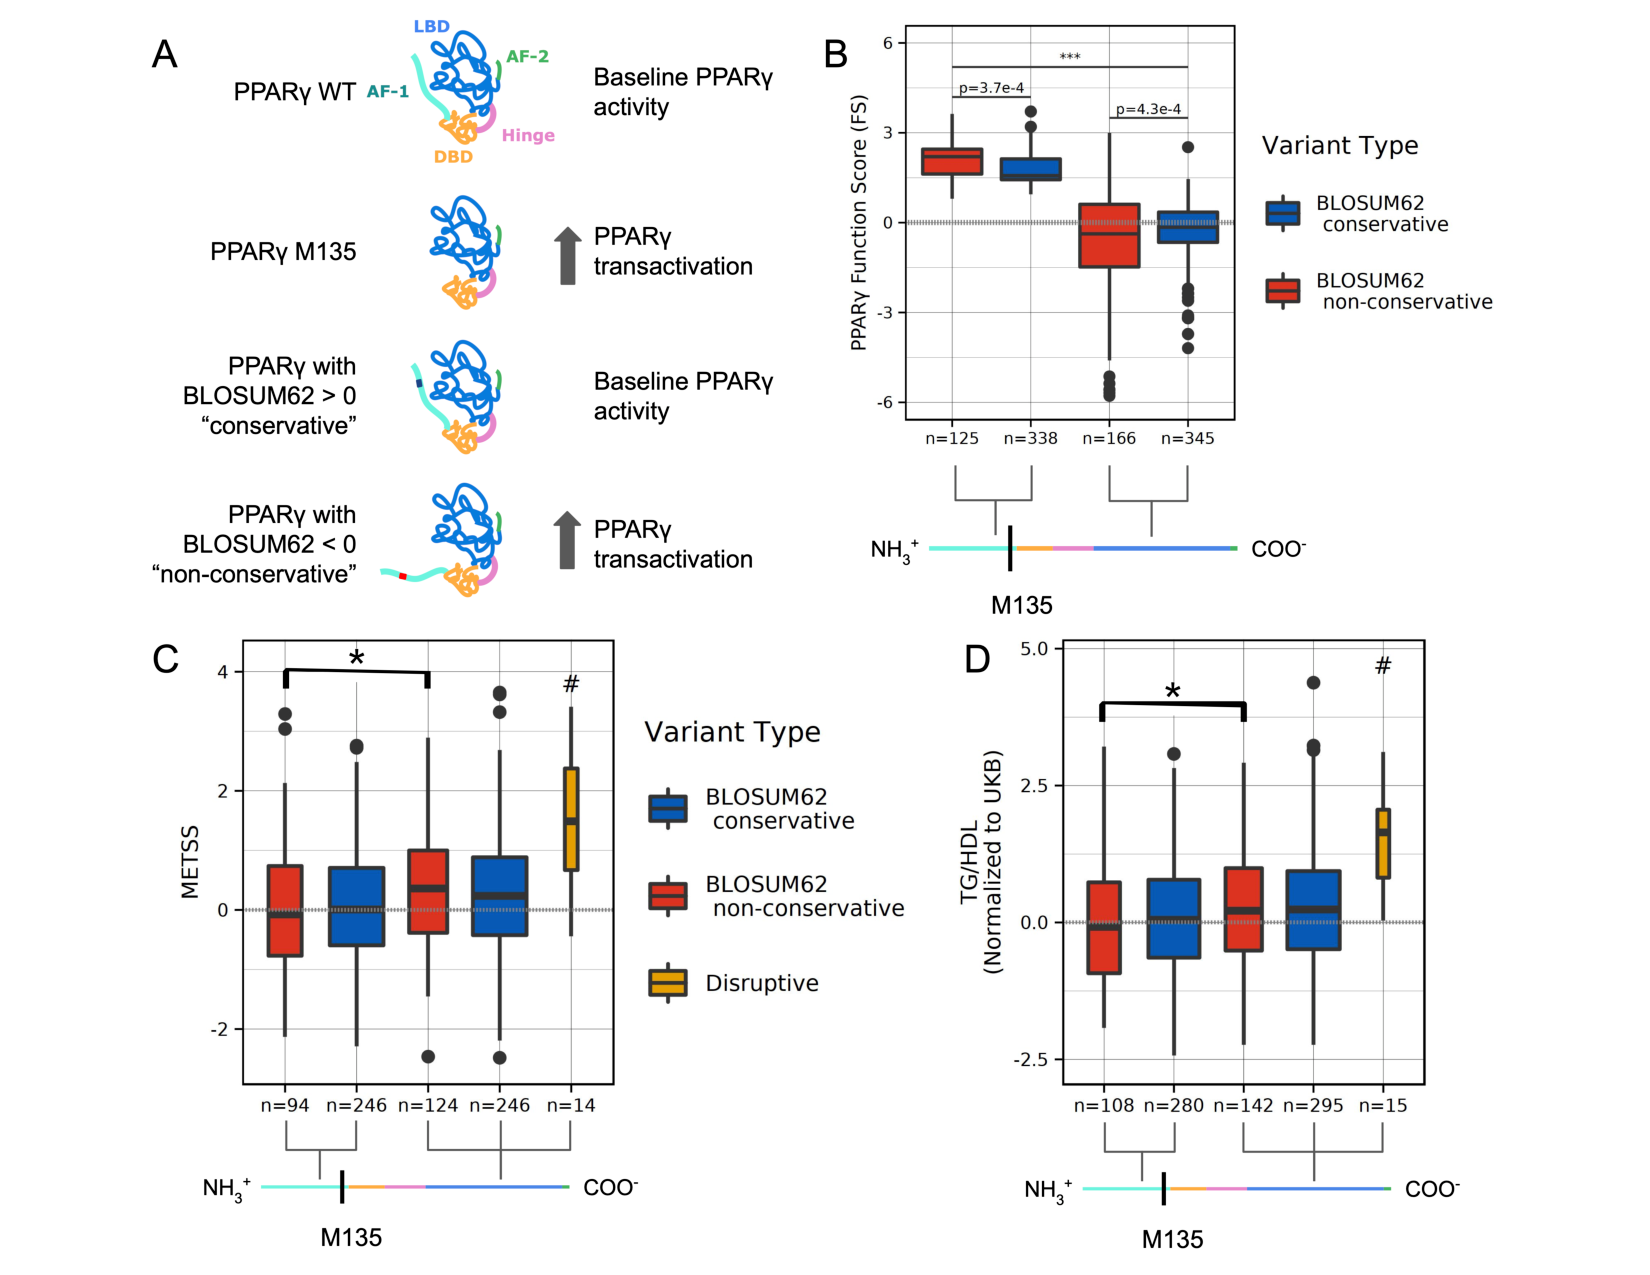
\includegraphics[width=\textwidth]{2_figures-and-files/Fig3.pdf}
    \caption[Human carriers of variants in PPAR$\gamma$ that impair the AF-1 domain are protected from metabolic dysfunction.]{\textbf{Human carriers of variants in PPAR$\gamma$ that impair the AF-1 domain are protected from metabolic dysfunction.} \textbf{A.} Cartoon representation of AF-1 hypothesis. Cyan: AF-1, Orange: DNA-binding domain (DBD), Pink: Hinge, Blue: Ligand-binding domain (LBD), Green: AF-2. Protein cartoon modeled after the PPAR$\gamma$ crystal structure shown in Mosure et al., 2022. \textbf{B.} Function scores (FS) for \(PPARG\) missense variants (MAF $<$ 0.001) from the UK Biobank (UKB) by position (i.e. pre-/post-M135), and evolutionary conservation (conservative: BLOSUM62 $<$ 0, nonconservative: BLOSUM62 $>$ 0) category. All pairwise comparisons between categories are significant by ANOVA (p $<$ 2e-16, ***) and Tukey HSD. \textbf{C.} Metabolic syndrome severity score (METSS) by position and conservation, as in B. There is a significant difference between pre-/post-M135 non-conservative METSS (*, p=0.016, Welch’s t). \# indicates that the disruptive carriers are significantly different from every other category by ANOVA (p=4.1e-6) and Tukey HSD (p$<$8.6e-4). \textbf{D.} TG/HDL, a measurement for insulin resistance, is plotted by position and conservation. The carriers of disruptive variants have significantly higher TG/HDL (\#, ANOVA p=7.31e-7, Tukey HSD p$<$1.1e-4), and there is a significant difference between pre-/post-M135 non-conservative variant carriers (*, p=0.017, Welch’s t).
    }\label{fig:Human carriers of PPARG variants}
\end{figure}
\clearpage

We identified all carriers of rare (MAF $<$ 0.001) protein-coding variants in \(PPARG\) in the UK Biobank (UKB, n=454,787)\cite{Backman2021-kd} and analyzed the cellular function and amino acid position of the variants carried in relation to the insulin sensitivity-related phenotypes of the individuals carrying them. To quantify PPAR$\gamma$ activity, we leveraged the PPAR$\gamma$ function score (FS) derived from our previously published deep mutational scan, in which every possible missense variant was scored by its transactivation of CD36\cite{Majithia2016-bm}. We found 1,250 carriers of 260 unique rare, protein-coding \(PPARG\) variants and partitioned them by pre-/post- M135 and by the BLOSUM62 substitution matrix, which quantifies the tolerance of amino acids to substitution across evolutionary distance\cite{Henikoff1992-jo}. Variants were categorized as “conservative” (BLOSUM62 $>$ 0) or “non-conservative” (BLOSUM62 $<$ 0). Non-conservative substitutions in AF-1 ($\mathrm{FS}_{\mathrm{median}}$=2.21) have higher PPAR$\gamma$ FS than conservative substitutions ($\mathrm{FS}_{\mathrm{median}}$=1.56), while non-conservative substitutions post-M135 in the DBD and LBD ($\mathrm{FS}_{\mathrm{median}}$=-0.158) show decreased PPAR$\gamma$ FS relative to conservative mutations ($\mathrm{FS}_{\mathrm{median}}$=-0.376; ANOVA p$<$2e-16, adjusted p$<$0.005 for each pairwise comparison by Tukey HSD; \textbf{Figure 2.3B}). These data support the hypothesis that missense variants disrupting AF-1 domain function increase the transcriptional activity of PPAR$\gamma$.

To quantify insulin sensitivity in these \(PPARG\) missense variant carriers, we computed a per-individual metabolic syndrome severity score (METSS), a measure of insulin sensitivity determined from waist circumference, systolic blood pressure, serum triglycerides, HDL cholesterol, and serum glucose (HbA1c), using methods analogous to those previously published\cite{Gurka2014-ib,Cavero-Redondo2019-ce,Agarwal2012-qu}. We calculated METSS for the 368,911 individuals in the UKB who had all five measurements ascertained, including 908 of the 1250 carriers of rare, protein-coding \(PPARG\) variants (\textbf{Figure B.1a, b}). Of the rare \(PPARG\) missense variant carriers in the UKB, 340 pre-M135 and 370 post-M135 carriers had computable METSS values. As with the PPAR$\gamma$ function score analysis above (\textbf{Figure 2.3B}), we partitioned each group into conservative and non-conservative BLOSUM62 to examine the effect of each variant category on METSS (\textbf{Figure 2.3C}). Under the model that amino acid substitutions that abrogate AF-1 domain function would increase PPAR$\gamma$ activity and thereby decrease METSS, we hypothesized that non-conservative missense variants in AF-1 (pre-M135) would confer lower METSS as compared to conservative amino acid substitutions that would preserve AF-1 function. Conversely, we expected that non-conservative mutations post-M135 in the DBD or LBD would increase METSS, as is the case for lipodystrophy\cite{Jeninga2009-pt}. As a positive control, we identified carriers of post-M135 disruptive (i.e. nonsense and frameshift causing) \(PPARG\) variants (n=14) in our cohort and found their METSS score to be significantly elevated ($\mathrm{METSS}_{\mathrm{median}}$=1.5, \textbf{Figure 2.3C}) compared to other \(PPARG\) variant carriers (ANOVA p=4.1e-6, Tukey p$<$8.6e-4) and the general UKB population (Welch’s t, p=1.1e-4). We observed an ordinal trend with non-conservative, pre-M135 variant carriers having the lowest METSS ($\mathrm{METSS}_{\mathrm{median}}$=-0.079) followed by conservative, pre-M135 ($\mathrm{METSS}_{\mathrm{median}}$=0.0064), conservative, post-M135 ($\mathrm{METSS}_{\mathrm{median}}$=0.24) and finally non-conservative, post-M135 ($\mathrm{METSS}_{\mathrm{median}}$=0.36). The difference between pre- and post-M135 non-conservative variant carriers is significant (Welch’s t, p=0.016).

We performed a similar analysis alternatively utilizing the serum triglyceride to HDL cholesterol (TG/HDL) ratio as a surrogate measure of insulin sensitivity\cite{Oliveri2024-bz,DeForest2024-ex}. The trends observed with METSS were consistent in the TG/HDL results: carriers of post-M135 disruptive (i.e. nonsense and frameshift causing) \(PPARG\) variants (n=15) had the highest values compared to other \(PPARG\) variant carriers ($\mathrm{TG/HDL}_{\mathrm{median}}$=1.65, \textbf{Figure 2.3D}; ANOVA p=7.31e-7, Tukey HSD p$<$1.1e-4), and the non-conservative, pre-M135 variant carriers had the lowest TG/HDL (n=108, $\mathrm{TG/HDL}_{\mathrm{median}}$= +0.080). The difference between pre- and post-M135 non-conservative variant carriers is significant (Welch’s t, p=0.017).

\clearpage
\begin{table}[t]
    \centering
    \caption[METSS statistics for carriers of \texorpdfstring{\(PPARG\)}{PPARG} Pro12Ala (rs1801282) in the UKB.]{\textbf{METSS statistics for carriers of \texorpdfstring{\(PPARG\)}{PPARG} Pro12Ala (rs1801282) in the UKB.}  Increasing alleles of Ala are associated with decreasing METSS.
  }
    \begin{tabular}{|c|c|c|c|c|}
    \hline
        Genotype & Carriers (n) & Median METSS & Mean METSS & Standard Deviation \\ \hline
        Pro/Pro & 287785 & 0.0035 & 0.0087 & 1.0015 \\ \hline
        Pro/Ala & 75619 & -0.0326 & -0.026 & 0.9947 \\ \hline
        Ala/Ala & 5263 & -0.0839 & -0.0964 & 0.9796 \\ \hline
    \end{tabular}
\end{table}

We separately analyzed the well known \(PPARG\) p.P12A variant (rs1801282, MAF=\newline 0.1050) that is associated with decreased type 2 diabetes risk\cite{Altshuler2000-kl} and occurs frequently in the general population. Under the above partitioning scheme, \(PPARG\) p.P12A would be classified as pre-M135, non-conservative (FS = 1.3, BLOSUM62 score = +1). Carriers of the p.P12A allele (n=80,882) in the UKB had significantly decreased METSS (per allele effect size = +0.039, p=2e-16, \textbf{Table 2.1}, \textbf{Figure B.1c}). These data are suggestive of a model in which AF-1 disrupting variants (both common and rare) can improve insulin sensitivity in vivo.


%%%%%%%%%%%%%%%%%%%%%%%%%%%%%%%%%%%%%%%%%%%%%%%%%%%%%%%%%%%%%%%%%%%%%%%%%%%%%%%%
\section{Discussion}
%%%%%%%%%%%%%%%%%%%%%%%%%%%%%%%%%%%%%%%%%%%%%%%%%%%%%%%%%%%%%%%%%%%%%%%%%%%%%%%%

In this study, we characterize the function of PPAR$\gamma$ M135 in adipocytes and model its effects with human genetics. We show that PPAR$\gamma$ M135 is more transcriptionally active and insulin sensitizing than WT PPAR$\gamma$ in response to exogenous agonism in human preadipocytes. Finally, we characterize metabolic syndrome severity in human carriers of \(PPARG\) variants, demonstrating that variants that abrogate AF-1 domain function potentially protect carriers from insulin resistance. Our data support a model for in vivo de-repression of PPAR$\gamma$ in humans that is metabolically beneficial.  

Regarding therapeutic development, our data suggest an opportunity to physiologically activate PPAR$\gamma$ through a mechanism distinct from thiazolidinediones (TZDs), which bind the LBD. While TZDs have demonstrated benefits in treating/preventing type 2 diabetes and CVD events\cite{Lebovitz2019-oe,dreamteam2006-hz}, they cause side effects such as weight gain\cite{Yki-Jarvinen2004-ba}. Much pharmacological development has focused on identifying molecules that are selective PPAR$\gamma$ modulators (SPPARMs) that would provide insulin sensitization without side effects, but most SPPARM molecules target the LBD of PPAR$\gamma$\cite{Higgins2010-tv} and still show appreciable rates of weight gain and fluid retention compared to placebo\cite{DePaoli2014-hi}. Our study nominates the AF-1 domain as a therapeutic target that is mechanistically distinct from TZDs and SPPARMs, as removing the AF-1 would de-repress rather than activate PPAR$\gamma$. Accordingly, our data show that adipocytes engineered to produce PPAR$\gamma$ M135 express higher levels of adiponectin, an insulin sensitizing adipokine\cite{Berg2001-oq,Stern2016-kw}. Further supporting this proposal are the murine models of human and synthetic \(PPARG\) variants that increase PPAR$\gamma$ activity via impairing AF-1 (p.P12A\cite{Heikkinen2009-vb}, p.S112A\cite{Rangwala2003-hm}, p.K107\cite{Katafuchi2018-jw}) which show enhanced insulin sensitivity compared to WT littermates.

In summary, we report on PPAR$\gamma$ M135, a novel isoform of \(PPARG\) arising from a downstream alternative translational start site (chr3:12381414 hg38), that is a more potent ligand-inducible transactivator than full-length PPAR$\gamma$. This work points to a new mechanism to activate PPAR$\gamma$ by inhibition of the AF-1 domain that could potentially lead to more effective treatments for insulin resistance-related disorders.

%%%%%%%%%%%%%%%%%%%%%%%%%%%%%%%%%%%%%%%%%%%%%%%%%%%%%%%%%%%%%%%%%%%%%%%%%%%%%%%%
\section{Research Design and Methods}
%%%%%%%%%%%%%%%%%%%%%%%%%%%%%%%%%%%%%%%%%%%%%%%%%%%%%%%%%%%%%%%%%%%%%%%%%%%%%%%%

\subsection{Generation and characterization of SGBS cell lines edited at the \texorpdfstring{\(PPARG\)}{PPARG} locus}

SGBS cells were seeded at 10,000 cell/cm2 and transduced with the endonuclease Cas9 and guides Int-sgRNA, Ex1-sgRNA2, and Ex3-sgRNA. Infected cells were selected with puromycin and differentiated 7 days after infection as we have previously published\cite{Jiao2019-ng}. Staining and quantification of cells for lipid accumulation with BODIPY (lipid) and DAPI (nuclei) after differentiation was performed as we have done previously\cite{Majithia2014-op}. Quantitative PCR for day 4 differentiation was performed as detailed above for THP-1s. Data were analyzed in aggregate over two separate transductions (batches), each with three biological replicates. To account for multiple biological replicates in two separate batches, relative expression (fold-change) was determined by a linear model of $\Delta$Ct \textasciitilde Genotype (Int, Ex1, Ex3) + Transduction\_Batch, using the intronic targeted samples as reference (i.e. calibrator). The estimate, error, and p-values for Genotype were used as the $\Delta\Delta$Ct, standard error, and p-values, respectively, with relative expression calculated as \[2^{-\Delta\Delta\mathrm{Ct}}.\]

\subsection{SGBS rescue experiments}

\(PPARG\) cDNA was synthesized (Twist Bioscience) with synonymous mutations\newline (CCDS2609 c.C594T, c.G603C, c.T610A, c.C511G) to eliminate the Ex3-sgRNA recognition sequence (chr3:12392727-12392749), following the principles of guide-intrinsic mismatch tolerance\cite{Fu2022-jh}. The oligo was PCR amplified to generate cDNA sequences encoding PPAR$\gamma$2 and PPAR$\gamma$ M135. These sequences were cloned into the doxycycline-inducible pCW plasmid (Addgene \#184708) using AgeI-HF (NEB \#M0202S), NheI-HF (NEB \#R3131S), and T4 DNA ligase (NEB \#M0202S). Virus was produced, and SGBS P$\gamma$-/- cells were infected to create the SGBS P$\gamma$-/- +WT and SGBS P$\gamma$-/- +M135 cell lines. Cells were differentiated for 12 days before downstream experiments.

\subsection{Imaging}
Cells were fixed in 4\% PFA for 10 minutes (Fisher Scientific \#50-980-487), permeabilized with 0.1\% Triton X-100 (Sigma Aldrich \#X100) for 10 minutes, then stained with 5 ug/mL DAPI (Sigma Aldrich \#D9542) and 2 ug/mL BODIPY 493/503 (Invitrogen \#D3922) for 30 minutes. Images were acquired using a Nikon BioPipeline spinning disk confocal microscope and analyzed using CellProfiler v4.1.3\cite{Carpenter2006-vm}.

\subsection{Insulin Stimulation}
Day 12 SGBS adipocytes were cultured in insulin-free DMEM F12 for 24 hours prior to stimulation with 100 nM recombinant insulin (Sigma Aldrich \#I9278) for 20 minutes in glucose-free Krebs-Ringer buffer as previously described\cite{Tews2022-am}. Cells were placed on ice and insulin-containing buffer was immediately removed prior to washing with cold PBS and cell collection.

\subsection{Immunoblots for phosphorylated-Akt (pAkt) and Akt}
Protein lysates for the SGBS adipocytes were processed as detailed above, and the membranes were incubated with primary antibodies CST \#2920 (Akt), CST \#4060 (phospho-Akt Ser473), and CST \#43603 (cyclophilin B), followed by fluorescent secondary antibodies CST \#5366, \#5151, and \#5470. Imaging was performed on the Odyssey CLx imager (LI-COR).

\subsection{Human Biobank Data}
UK Biobank (UKB) research was conducted under application numbers 41189 and 51436. Framingham Heart Study (FHS) data was accessed through dbGaP project \#30824, “Study on Genetic Risk Scores for Insulin Resistance and their Relation to Metabolic Diseases,” and the All of Us Researcher Workbench was accessed through the workspace, “Detection and analysis of genetic risk factors for insulin resistance v7.” The 1000G variants were accessed through the public data browser\cite{1000_Genomes_Project_Consortium2015-fz}. The Regeneron Genetics Center Million Exome dataset was accessed through the public variant browser\cite{Sun2023-ty}, which includes data accessed through UKB application 26041. The Regeneron Genetics Center, and its collaborators (collectively, the “Collaborators”) bear no responsibility for the analyses or interpretations of the data presented here. Any opinions, insights, or conclusions presented herein are those of the authors and not of the Collaborators. For all exome sequenced cohorts, variants within the genomic coordinates of \(PPARG\) (chr3: 12287368-12434356 hg38) were extracted, and variant annotation was performed using SnpEff v4.3\cite{Cingolani2012-gd}. Nomenclature used for missense variants is for the canonical \(PPARG\) transcript ENST00000287820.10; protein ENSP00000287820.6. Function scores were obtained from the \(PPARG\) saturation mutagenesis performed by Majithia et al.\cite{Majithia2016-bm}.

\subsection{Metabolic syndrome severity score (METSS)}
To calculate a continuous score for metabolic syndrome severity, the values of the five constituent clinical phenotypes\cite{Gurka2014-ib,Cavero-Redondo2019-ce}, serum HDL cholesterol (field 30760), waist circumference (field 48), serum triglycerides (field 30870), systolic blood pressure (field 4080), and glycated hemoglobin (HbA1c, field 30750), were extracted for all UKB participants who had a complete set of measurements and genetic ancestry data (n=368,911). Systolic blood pressure values were corrected for individuals reported to be taking blood pressure medication by adding 15 mm Hg to the listed measurements\cite{Evangelou2018-wo}, and serum triglyceride values were log-normalized. To incorporate the multiple parameters that define metabolic syndrome into one score, dimensionality reduction through principal component analysis (R 4.1.3 prcomp) was performed on the corrected values of the five phenotypes. The resulting principal components (PCs) were regressed against PPAR$\gamma$ function score (FS), adjusted for age, $\mathrm{age}^2$, and sex, and the significant PCs were combined into the metabolic syndrome severity score (METSS = PC5 + PC4 + PC1). The score was adjusted for the covariates of age, age2, sex, and the first ten principal components of genetic ancestry, and the residuals were normalized across the UKB participants (n=368,911). The final METSS thus has a mean of 0 and standard deviation of 1 across the UKB, and it has a significant effect size when regressed against the PPAR$\gamma$ FS (\textbf{Figure B.1b}).

\subsection{TG/HDL}
Serum HDL cholesterol (field 30760) and serum triglycerides (field 30870) were extracted for all UKB participants who had a complete set of measurements and genetic ancestry data (n=425,472). Serum triglyceride values were log-normalized, and the ratio of TG/HDL was applied. TG/HDL was adjusted for the covariates of age, $\mathrm{age}^2$, sex, and the first ten principal components of genetic ancestry, and the residuals were normalized across the UKB participants (n=425,472).

%%%%%%%%%%%%%%%%%%%%%%%%%%%%%%%%%%%%%%%%%%%%%%%%%%%%%%%%%%%%%%%%%%%%%%%%%%%%%%%%
\section{Acknowledgements}
%%%%%%%%%%%%%%%%%%%%%%%%%%%%%%%%%%%%%%%%%%%%%%%%%%%%%%%%%%%%%%%%%%%%%%%%%%%%%%%%
We would like to thank the All of Us participants, as the All of Us Research Program would not be possible without their partnership. We are grateful to Angela Liu for technical assistance. Microscopy was performed at the Nikon Imaging Center at UCSD with the support of P. Guo and R. Sanchez. This research has been conducted using the UK Biobank Resource under Application Numbers 41189 and 51436. We would like to acknowledge the participants and the contributions made by the UK Biobank (www.ukbiobank.ac.uk) in providing the data and resources used in this study.  

\subsection{Author Contributions}
As this work was derived from the same manuscript, see \ref{chap:chapter 1} for corresponding details.

\subsection{Funding}
This work was supported by grants from the National Institute of Diabetes and Digestive and Kidney Diseases (1R01DK123422 and R01HL159760 to A.R.M, 1R01DK125490 to J.F and A.R.M) and a UCSD/UCLA Pilot and Feasibility grant (P30 DK063491 to A.R.M). This publication includes data generated at the UC San Diego IGM Genomics Center utilizing an Illumina NovaSeq 6000 that was purchased with funding from a National Institutes of Health SIG grant (\#S10 OD026929). The All of Us Research Program is supported by the National Institutes of Health, Office of the Director: Regional Medical Centers: 1 OT2 OD026549; 1 OT2 OD026554; 1 OT2 OD026557; 1 OT2 OD026556; 1 OT2 OD026550; 1 OT2 OD 026552; 1 OT2 OD026553; 1 OT2 OD026548; 1 OT2 OD026551; 1 OT2 OD026555; IAA \#: AOD 16037; Federally Qualified Health Centers: HHSN 263201600085U; Data and Research Center: 5 U2C OD023196; Biobank: 1 U24 OD023121; The Participant Center: U24 OD023176; Participant Technology Systems Center: 1 U24 OD023163; Communications and Engagement: 3 OT2 OD023205; 3 OT2 OD023206; and Community Partners: 1 OT2 OD025277; 3 OT2 OD025315; 1 OT2 OD025337; 1 OT2 OD025276.
\\

\noindent Chapter 2, in full, was modified for this thesis from the material in Diabetes 2025. The dissertation/thesis author was the primary investigator and author of this paper. I would like to acknowledge my co-authors for the research in Chapter 2, Karen Mendez-Lara, Siqi Hu, Rachel Diao, Guru Bhavimani, Ruben Hernandez, Kimberly Glass, Camila De Arruda Saldanha, Jason Flannick, Sven Heinz, and Amit Majithia.

\bibliographystyle{unsrtnat}
\bibliography{bib_2.bib}